%----------------------------------------------------------------------------
%----------------------------------------------------------------------------
We measure the RF spectrum of two dye lasers (\#22 and \#23) using two receivers (the 7L12 and the 7L14). Selection between the two laser sources is facilitated through the use of a mirror mounted on a magnetic kinematic base (called the ``switch'' in Fig. \ref{block}).
%----------------------------------------------------------------------------
%----------------------------------------------------------------------------
%bb defines the bounding box for the pdf
%----------------------------------------------------------------------------
\begin{figure}
\scalebox{0.65}[0.65]{
\includegraphics*[bb=55 87 640 383]
{block/block.pdf}
}
\caption[Block diagram RF beat spectrum measurement]{Block diagram RF beat spectrum measurement. The connection between the computer and the RF receiver (which carries the voltage ramp that scans the receiver) is not shown here.}
\label{block}
\end{figure}
%----------------------------------------------------------------------------

%----------------------------------------------------------------------------
When the mirror is in place and the beam from dye \#23 blocked, the beam from dye \#22 is directed toward the photodiode. When the mirror is removed, the beam from dye \#23 is incident on the photodiode. Switching between laser sources takes seconds. To attenuate the beam down to appropriate levels for the photodiode, the laser output is reflected off the front surface of a wedged quartz plate - the rear surface reflection is directed toward a beam dump while the front surface reflection is directed through two crossed polarizers and three neutral density filters (ND 0.3, 0.7, and 2.0). After the ND filters the beam is incident on the photodiode.

Before being analyzed by the receiver, the electronic signal from the photodiode is sent through a high pass filter (see Fig. \ref{highpass}
%----------------------------------------------------------------------------
%----------------------------------------------------------------------------
%bb defines the bounding box for the pdf
%viewport defines the area of the pdf used
%in sidewaysfigure the last entry in bb moves the caption toward/away the pic
%in sidewaysfigure the second entry in bb moves the pic toward/away the caption
%----------------------------------------------------------------------------
\begin{figure}
\begin{center}
\leavevmode
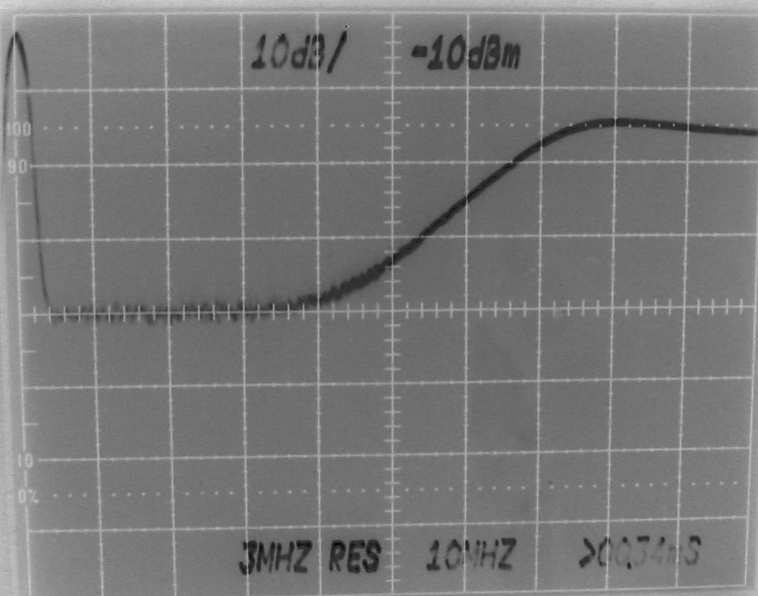
\includegraphics[width=3.5in]
{highpass/highpass.png}\\
\end{center}
\caption[Highpass filter response]{Highpass filter response. The output of the tracking generator was feedback into the RF receiver through the highpass filter while the receiver self-scanned. We see the filter begins to pass significant power at 50 MHz and reaches 100\% transmission at 75 MHz.}
\label{highpass}
\end{figure}
%----------------------------------------------------------------------------

%----------------------------------------------------------------------------
 for the response curve for the filter). A 14 dB attenuator is placed between the photodiode and the filter to minimize back reflections from the filter (see Fig. \ref{filter}
%----------------------------------------------------------------------------
%----------------------------------------------------------------------------
%bb defines the bounding box for the pdf
%viewport defines the area of the pdf used
%in sidewaysfigure the last entry in bb moves the caption toward/away the pic
%in sidewaysfigure the second entry in bb moves the pic toward/away the caption
%----------------------------------------------------------------------------
\begin{figure}
\begin{center}
\leavevmode
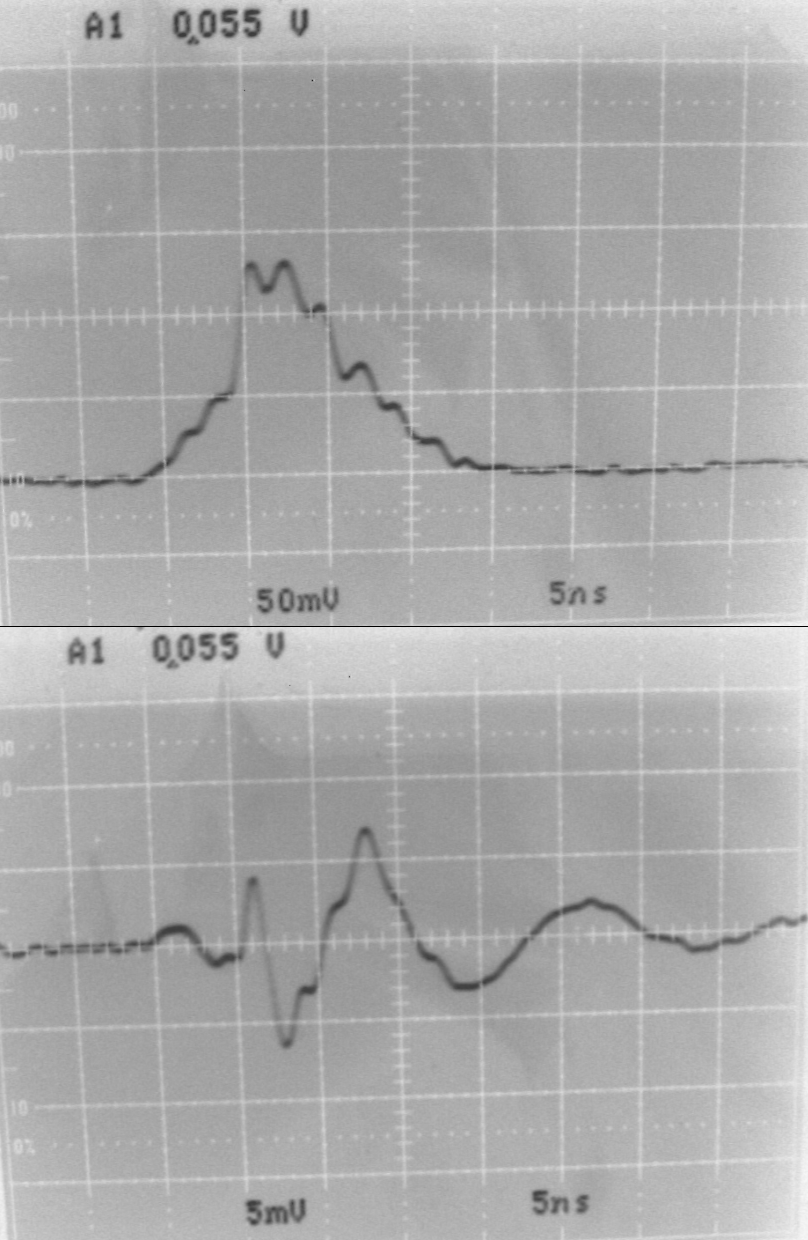
\includegraphics[width=4in]
{filter/filter.png}\\
\end{center}
\caption[Photodiode signal through the highpass filter (and 14 dB attenuator)]{Photodiode signal through the highpass filter (and 14 dB attenuator). The upper photo shows a typical signal from the photodiode after a dye laser pulse is detected. The lower photo shows a typical signal after the insertion of the 14 dB attenuator and the highpass filter between the photodiode and the oscilloscope.}
\label{filter}
\end{figure}
%----------------------------------------------------------------------------

%----------------------------------------------------------------------------
for the effect of the attenuator and filter on an actual pulsed signal from the photodiode). The SR250, triggered by the light scattered from the beam dump, gates and averages the receiver output. A laptop computer using the ``voltage ramp chart recorder'' LabView program (see AHI00-TP3300-01-VR03) simultaneously samples the boxcar integrator output and supplies a voltage ramp to the receiver. The voltage ramp scans the receiver across most of its usable range.
%----------------------------------------------------------------------------
%----------------------------------------------------------------------------
